\documentclass[12pt]{book}

\usepackage[colorlinks=true,linkcolor=black,citecolor=blue,pdfusetitle]{hyperref}
\usepackage{cite}
\usepackage[nonumberlist]{glossaries}
\usepackage[utf8]{inputenc}     % UTF8 characters in .tex docs
\usepackage{graphicx}

\pdfinfo{ % This just add some details to the file metadata
    /Title (Use of an Optical Dipole Trap in a Cold-atom Electron Source)
    /Author (Joshua Torrance joshuatorrance@gmail.com)
    /Subject (MSc Thesis)
    /Keywords (physics, atoms, Rubidium, lasers, masters)
    }

\newacronym{cdi}
    {CDI}{coherent diffractive imaging}

\newacronym{odt}
    {ODT}{optical dipole trap}

\newacronym{bec}
    {BEC}{Bose-Einstein condensate}

\newacronym{fort}
    {FORT}{far-off-resonance trap}

\makeglossaries

\title{Use of an Optical Dipole Trap in a Cold-atom Electron Source}
\author{Joshua Torrance}
\date{\today}

\begin{document}

\pagenumbering{gobble}  % so the title page isn't numbered
%\maketitle


%%% Title page %%%
    \renewcommand{\footnotesize}{\small}
    \renewcommand{\footnoterule}{\relax}
    \thispagestyle{empty}
    \begin{center}
        { \Huge {\bfseries {Use of an Optical Dipole Trap in a Cold-atom Electron Source}} \par}
    {\large \vspace*{35mm} {{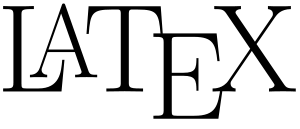
\includegraphics[width=4cm]{figs/logo.png}} \par} \vspace*{25mm}}
        {{\vspace*{30mm} \Large {Joshua Torrance}} \par} 
    {\large 
	    \vspace*{1ex}
        {{School of Physics} \par}
	    \vspace*{1ex}
        {{The University of Melbourne} \par}
	    \vspace*{25mm}
    }%end large
    \end{center}
    \null\vfill

\tableofcontents
\pagenumbering{roman}

\renewcommand{\chaptername}{} % uncomment to print only "1" not "Chapter 1"


\chapter{Introduction}
\pagenumbering{arabic} % This works correctly if it's here

The University of Melbourne's \gls{caes} project aims to create short, high-brightness, high-coherence electron bunches for use in ultra-fast, single-shot \gls{cdi}. The imaging of nanoscale objects such as biological molecules \cite{dwyer_femtosecond_2006, williamson_clocking_1997} and defects in solid-state devices \cite{siwick_atomic-level_2003} by ultrafast, single-shot electron diffractive imaging would provide important information about structure and dynamic processes.

\section{Imaging of Bio-molecules}

In order to determine the structure of biological molecules, imaging techniques with atomics resolution are required. A number of techniques are capable of determining these structures \cite{nettleship_methods_2008, svergun_small-angle_2003, opella_structure_2004} and the most successful to date has been x-ray crystallography \cite{kendrew_three-dimensional_1958, uson_advances_1999}. Unfortunately the crystallisation process required for x-ray crystallography is difficult and to date only a small proportion of proteins have been successfully crystallised \cite{geerlof_impact_2006}.

Membrane proteins are proteins that are associated with or attached to the membranes of cells. They are involved in detecting and conveying external signals into cells. This allows the cells to interact with and respond to their environment\cite{almen_mapping_2009}. Membrane proteins are important in determining immune responses, interactions with pharmaceuticals, cell adhesion to form tissues and controlling important metabolic processes such as salt balance, energy production and photosynthesis\cite{chiras_human_2011}.

Determining the structure of theses molecules is a key step in understanding their chemical and biological function as well as how they will respond to drugs. The importance of knowing the atomic structure of biomolecules is exemplified by the enormous progress made in various fields of biology once the double-helical structure of DNA was determined from x-ray images in 1953 \cite{watson_molecular_1953}. Once a protein's structure and function are known then it becomes possible to design targeted drugs \cite{pinto_influenza_1992} and to more fully understand how the protein behaves in its biological system.

The development of new imaging techniques, such as ultrafast single shot diffraction, and new light sources, such as \glspl{xfel}, have been driven by the goal of overcoming the limitations of x-ray crystallography. Ultrafast single-shot diffraction imaging also has the potential to determine the dynamic structure of biological molecules.


\subsection{Ultrafast, single-shot, coherent diffractive imaging with electrons}

X-ray diffraction from crystals was first observed a century ago\cite{bragg_x-rays_1912} and resulted in a Nobel prize being awarded to William Henry Bragg and his son, William Lawrence Bragg. Since then a number of imaging techniques, such as \gls{cdi}, have been developed. \Gls{cdi} has been performed on a myriad of different samples with coherent beams of x-rays and electrons.

Ultrafast, single-shot imaging requires a very bright source of radiation in order to provide enough scattered information on the detector before the sample is damaged by the illumination\cite{henderson_potential_1995}. Single-shot imaging with a sufficiently bright source and a short enough interaction time would be able to image protein molecules, and other bio-molecules, without the need for crystallisation\cite{neutze_potential_2000}.

With femtosecond timescale single-shot imaging it is possible to observe dynamical systems such as molecular vibration and chemical reactions\cite{zewail_4d_2006}. With the sophisticated imaging techniques currently in development around the world and the continued improvement of radiation sources it will become possible to create `molecular movies'\cite{dwyer_femtosecond_2006} of these processes. Unfortunately, the brightnesses required for single shot imaging with x-rays requires multi-billion-dollar \gls{xfel} facilities.

Electron sources however may be able to provide a cheaper alternative. Electron interactions with molecules are significantly stronger than those of x-rays. For similar energies the electron interaction with a sample is $10^5-10^6$ times stronger than that of x-rays\cite{sciaini_femtosecond_2011}. This means that while a huge facility is required to generate x-ray light of sufficient brightness a table-top source of electrons may be sufficient for ultrafast \gls{cdi}.

\Gls{cdi} requires that the source have a coherence length greater than the length of the structures under investigation. For a quasi-homogeneous electron bunch the transverse coherence length, $L_c$, is\cite{van_oudheusden_electron_2007}
\begin{equation}
L_c = \hbar/\sqrt{m_e k_B T}.
\end{equation}
where $m_e$ is the mass of an electron and $T$ is the temperature of the electrons. The problem with conventional electron sources (such as electron guns, photocathode sources and field emission sources) is the temperature of the electrons produced. Most electron sources produce electrons with high temperatures which results in low coherence lengths and are thus not appropriate for \gls{cdi}. However the procedure used in the \gls{caes} results in low temperature electron bunches which are suitable for \gls{cdi}. The \gls{caes} also provides the ability to mitigate expansion due to space charge effects with electron bunch shaping\cite{mcculloch_arbitrarily_2011}.

The Melbourne optics group has recently shown that \gls{cdi} with electrons is possible, using a conventional electron microscope\cite{putkunz_atom-scale_2012}. The electron currents used are unfortunately too small for single-shot imaging.

\section{Melbourne cold-atom electron source}

If bright, coherent, femtosecond long bunches of electrons can be produced from the Melbourne \gls{caes} then \gls{cdi} can be performed on a range of structures and eventually molecules.

In order to produce electrons in the \gls{caes} rubidium atoms are cooled and trapped in a retro-reflective \gls{mot} that is loaded from a Zeeman slower\cite{phillips_laser_1982, phillips_cooling_1987, bell_slow_2010}. The valence electrons of the trapped atoms are then ionised using a two-stage ionisation process. The ionisation process is tuned such that the electrons are given the minimum energy required to ionise ensuring that the electrons are `cold' (approximately $10\,\unit{K}$\cite{mcculloch_arbitrarily_2011}).

The cold electrons are accelerated out of the cloud by a uniform electric field generated by charged parallel plates, guided to the neighbouring sample chamber and focused onto the target sample. After passing through the sample the resulting diffraction pattern is recorded with an imaging detector and can then be used to determine the structure of the sample using standard \gls{cdi} inversion techniques.

During the ionisation and acceleration stage the magnetic and optical trapping must be turned off. The optical trapping interferes with the ionisation stage and the magnetic trapping would have extremely strong effects on the electron trajectories due to the low mass of the electrons. This means that during these phases, the atom cloud is no longer trapped and begins to undergo thermal expansion and fall due to gravity.

This cycle of trapping, ionisation, acceleration and imaging occurs with a frequency of $10\,\unit{Hz}$ during normal operation.

\section{Stability of the cold-atom electron source}

In its current state the \gls{caes} suffers from a number of technical issues that are preventing the observation of diffraction through samples. One of these issues is the instability of the position of the electron signal on the detector which is due to the instability of the atom cloud and the long turn-off time of the magnetic trapping which interferes with the electron trajectories.

During the standard $10\,\unit{Hz}$ cycle the atom cloud formed by the \gls{mot} has approximately $93\,\unit{ms}$ to fill. This does not provide enough time for the trap to saturate and the distribution of the atoms within the cloud varies from cycle to cycle as a result. The atom distribution also varies during a single cycle as atoms `slosh' within the trap. These issues are exacerbated when the trapping is turned off and the cloud begins to fall and expand.

This instability in the distribution of the atoms results in instability in the initial distribution of the electrons. This is apparent on the detector as shot-to-shot variations in the position of the electron beam. Mitigating this instability would allow averaging of many shots to improve the signal to niose ratio and determine diffraction to higher order, thus increasing the imaging resolution.

\section{Optical dipole traps}

\Glspl{odt} may prove to be the solution to this stability problem. An \gls{odt} consists of a focused, Gaussian laser beam that is detuned from the atomic resonances of the target atomic species. The atoms feel a force towards the high intensity regions of the laser that is, towards the centre of the beam and the focus.

\subsection{History of optical dipole trapping}
The use of the optical dipole force as a confining mechanism was first proposed by Askar'yan in 1962\cite{askaryan_effects_1962} for plasmas and neutral atoms. Ashkin successfully demonstrated the trapping of micron-size latex spheres suspended in water using a focused Gaussian lasers in 1970\cite{ashkin_acceleration_1970}. The first optical trapping of atoms was demonstrated by Chu et al. in 1986\cite{chu_experimental_1986} where an \gls{odt} was used to trap sodium atoms.

Since then \glspl{odt} have been used extensively in atom optics and have proven invaluable in the creation of \glspl{bec} and atom lasers.

\subsection{Optical dipole traps in the cold-atom electron source}

The main advantage of \gls{odt} for the \gls{caes} is trapping without magnetic fields or on-resonance lasers. This means that the atom-cloud can remain trapped during the ionisation and acceleration phases of electron generation. This should reduce the instability in the electron beam path.

\Gls{odt} also provide the opportunity to experiment with other techniques such as evaporative cooling to compress the atom-cloud and optical lattices\cite{fallani_bose-einstein_2005} to counter disorder induced heating\cite{gericke_disorder-induced_2003}.

\Glspl{odt} used in the \gls{caes} must meet several criteria in order to be useful:
\begin{itemize}
    \item The trap depth must be at least as deep as the temperature of the atoms in the \gls{mot} which is approximately $135\,\unit{\mu K}$. A trap depth of ten times the average temperature of the \gls{mot} atoms is normally considered adequate so as to trap the majority of the atoms in the trapping region. The trap depth is affected by the power, the detuning from resonance and the size of the beam.
    \item The lifetime of the trap must be in excess of the length of the  ionisation and acceleration phase which is not longer than $10\,\unit{ms}$. The lifetime of the trap is affected by the temperature of the atoms and the scattering rate of the trapping light field which is determined by the intensity of the light at the trap and the trap laser detuning from resonance.
    \item Ideally the size of the trap would encompass the entire \gls{mot} however this is impractical due to the limitations in the laser power available. The minimum size of the trap should be the size of the excitation region which is of order $500\,\unit{\mu m}$\cite{mcculloch_towards_2012}.
\end{itemize}

Two light sources were considered for the production of the \gls{odt}. The first is a $780\,\unit{nm}$ \gls{ecdl} seeded \gls{ta} tuned to a wavelength around $781\,\unit{nm}$ with an applicable power of $700\,\unit{mW}$. The second is a $1064\,\unit{nm}$, $20\,\unit{W}$ fibre laser.

The majority of modern \glspl{odt} use light sources similar to the $1064\,\unit{nm}$ $20\,\unit{W}$ fibre laser taking advantage of the extremely low scattering rates to get long lifetimes. The \gls{caes} however only requires the \gls{odt} for a few milliseconds so using the light source that is close to the atomic resonances may prove to be the better option.

This project focusses on the design and construction of a \gls{ta} source for an \gls{odt} to be used in the Melbourne \gls{caes}, the theory involved in created, imaging and analysing the \gls{odt}, the experimental setup of the Melbourne \gls{caes} and how the \gls{odt} has been integrated and imaged.





\chapter{Motivation for an optical dipole trap}

When extracting the ionised electrons from the atom cloud it is necessary to turn off the magnetic trapping fields and the magnetic fields of the Zeeman slower in order to prevent magnetic distortions of the electron bunch trajectory. This means that just before electron extraction the cloud is no longer trapped it begins to expand. The use of additional trapping mechanisms that do not interfere with the electron trajectories, such as an \gls{odt}, will help prevent this expansion. An \gls{odt} will also serve to stabilise the initial position of the electron bunches which tend to drift at present due to dispersal of currents, and hence magnetic fields, in the magnetic coils and their power supplies.

Using an \gls{odt} in this system should also allow an increase in the brightness and perhaps coherence of the source due to higher atom cloud densities during the ionisation process. For single-shot \gls{cdi} a combination of coherence and electron current is required in order for sufficient information to be captured in the resulting diffraction pattern.

\section{Coherence}
Unsurprisingly coherence is an important factor in \gls{cdi} since this technique relies on the interference of the diffracted waves. The transverse coherence length of a imaging beam must be approximately twice the width of the object being imaged\cite{spence_coherence_2004} in order to properly resolve structure.

For a quasi-homogeneous source\cite{nugent_coherent_2009}, the transverse coherence length $L_c$ can be related to the transverse momentum spread, and hence the temperature, through\cite{van_oudheusden_electron_2007}
\begin{equation}
L_c = \hbar/\sqrt{m_e k_B T}.
\end{equation}

The transverse coherence is determined solely from the temperature of the electrons which is proportional to the temperature of the electron source and the ionisation energy.

The coherence of the electron bunches could be increased with the sophisticated use of \glspl{odt} since the trap would serve to reduce the temperature of the atom cloud, and hence the electron bunches.

\section{Brightness}
Brightness is important in single-shot \gls{cdi} due to the need to maximise the scattered signal to ensure sufficient sampling of the specimen within the exposure time.

For the cold-atom source the transverse brightness at the source is given by\cite{reiser_theory_2008}
\begin{equation}
B_\perp = \frac{I_p m_e c^2}{4 \pi^2 \sigma_x \sigma_y k_B T},
\end{equation}
where $\sigma_x$ and $\sigma_y$ are the root mean squared source size along the respective axes, $I_p$ is the peak electron current and $T$ is the source temperature.

The brightness of an electron bunch can be increased by a reduction in the length of the bunch or by increasing the density. A short bunch is also necessary for ultrafast electron diffraction.

The use of an \gls{odt} will increase the density of the atom-cloud by trapping the otherwise expanding atom-cloud which will result in an increase of the electron bunch density and hence the brightness.

\chapter{Optical dipole trapping}

Overview of experimental setup should be before this.
Should I go into detail on MOT theory?

If so then:
\begin{itemize}
\item zeeman slower
\item optical mollasses
\item magnetic trapping
\item electron excitation and ionisation
\item dipole trapping
\end{itemize}

\chapter{Experiment}

The \gls{caes} at the University of Melbourne has been assembled over a number of years. The experimental cycle can be divided into several parts which will be briefly described in this chapter. Details on the setup of the optical dipole trap and absorption imaging as well as the experimental sequence are given here. More details of the various experimental apparatus can be found in the group's recent papers \cite{bell_slow_2010, mcculloch_arbitrarily_2011, saliba_spatial_2012} and theses \cite{mcculloch_towards_2012, sheludko_shaped_2010, saliba_partially_2011}. A schematic of the main experiment can be seen in figure \ref{fig:experiment}.

\begin{figure}[h]
\centering
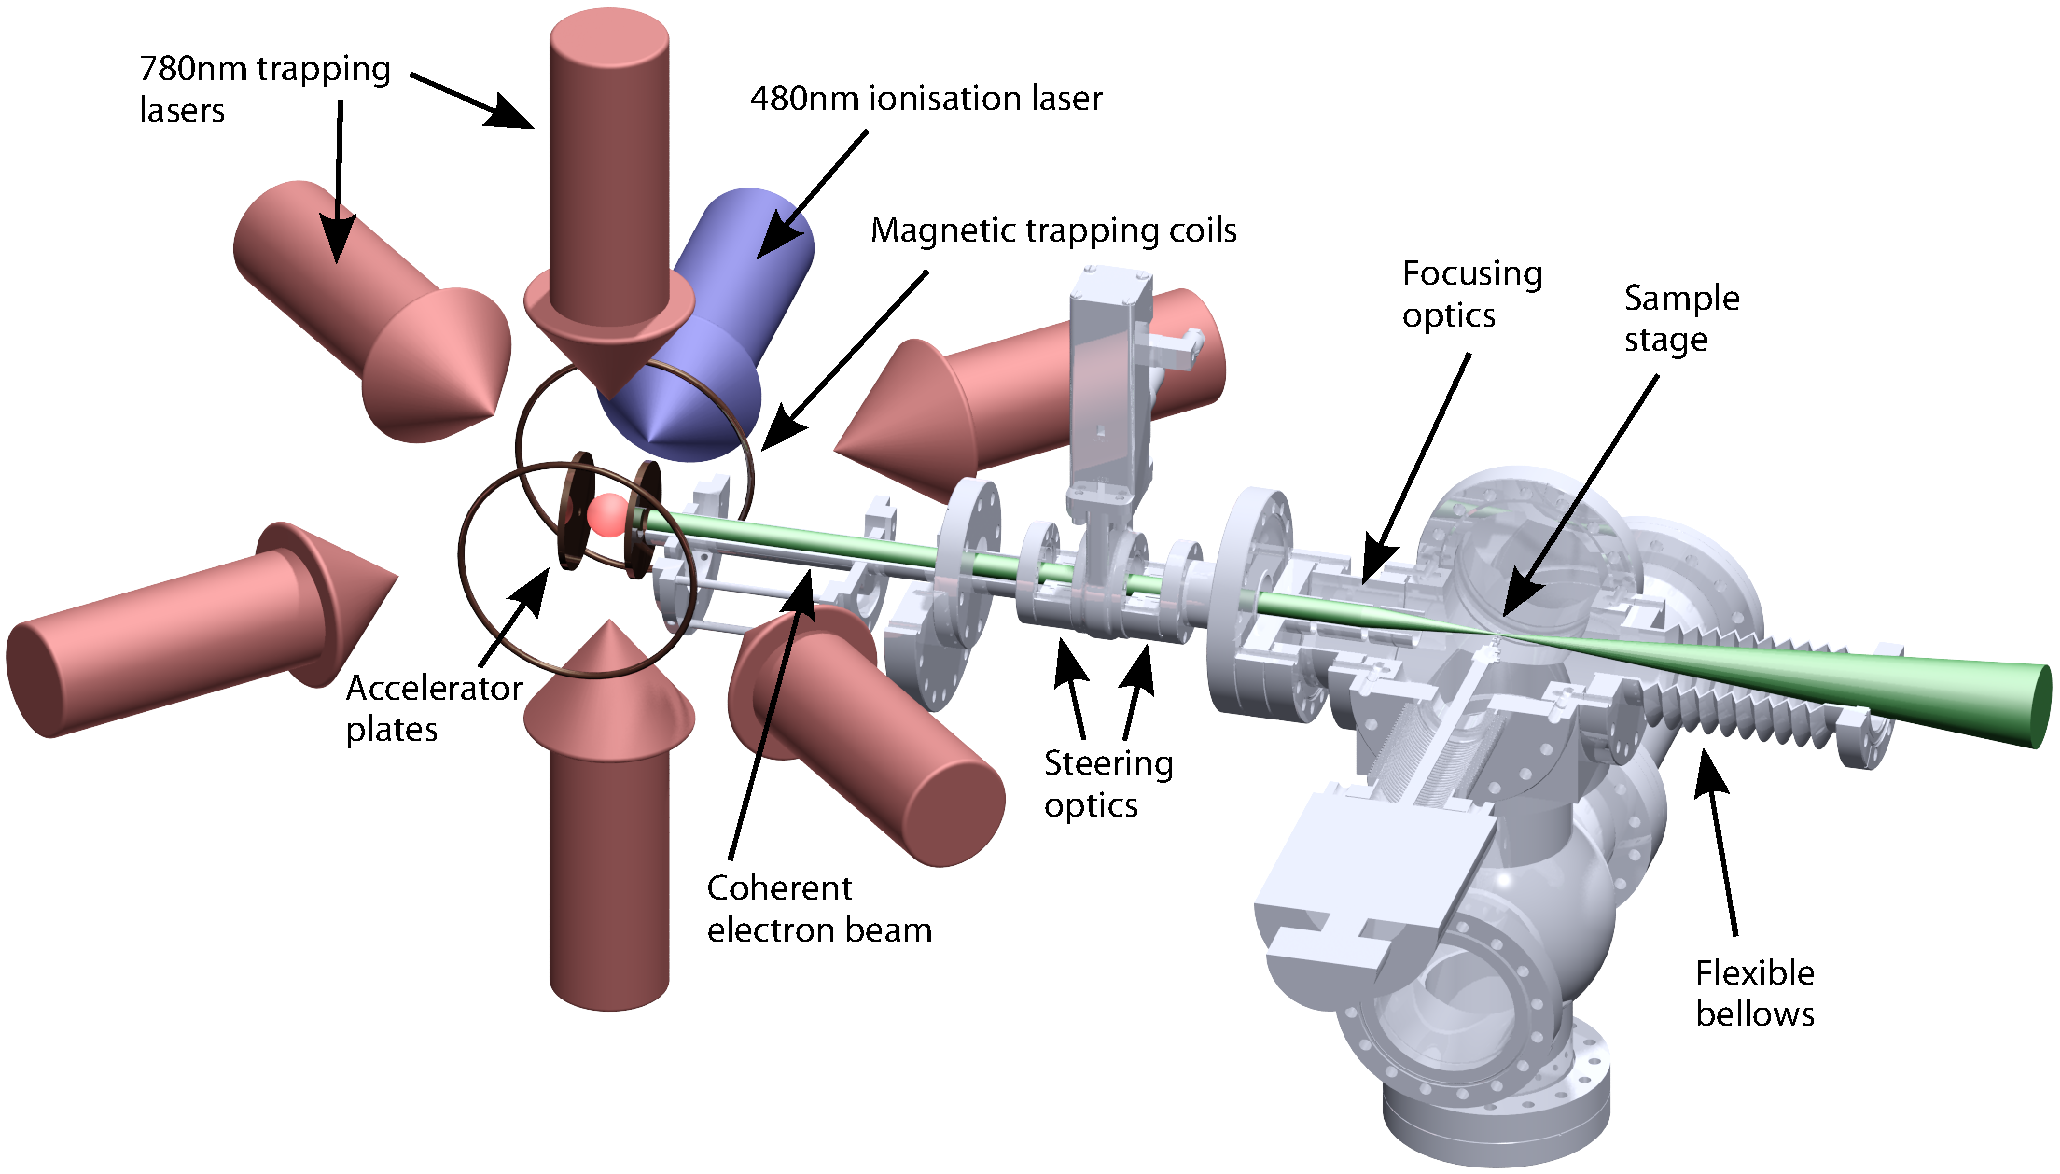
\includegraphics[width=0.75\textwidth]{figs/MOT_and_sample.pdf}
\caption{Laser cooled rubidium in a \protect\gls{mot} is ionised to form coherent electron pulses. These pulses are focussed onto a sample and the diffraction pattern is recorded.}
\label{fig:experiment}
\end{figure}

\section{Cold Atom Electron Source}
\subsection{Magneto-Optic Trap}
Rubidium atoms are trapped in a quasi-mirror \gls{mot} which is formed from three pairs of laser beams with $\sigma^\pm$ circular polarisation and wavelength $\lambda=780\,\unit{nm}$. The mirror-MOT configuration can suffer from reduced trapping volume\cite{reichel_atomic_1999} but in this case it is required to provide the accelerator structures. One of the accelerator plates is used as the mirror. Each of the \gls{mot} beams consists of both repump light and light detuned from the atomic resonance that is used for Doppler cooling.

The \gls{mot} is loaded from a tapered coil Zeeman slower which slows the hot atoms from the rubidium oven so that they can be trapped in the \gls{mot}. The light in the Zeeman slower also consists of both repump and cooling light.

\subsection{Ionisation}

In the \gls{caes}, ionisation is a two step process. The excitation can be performed with either a \gls{cw} $780\,\unit{nm}$ \gls{ecdl} or with an $800\,\unit{nm}$, femtosecond pulse laser. The femtosecond laser has the advantage of producing extremely short pulses of electrons however the electron temperature is higher\cite{mcculloch_high_2012}. A $480\,\unit{nm}$, $10\,\unit{ns}$ pulse laser is used to ionise the excited atoms. The ionisation laser shares its beam path through the vacuum system with the second beam of the crossed optical dipole trap.

The excitation lasers can both be shaped with an \gls{slm}. This shaping directly affects the shape of the electron bunches\cite{mcculloch_arbitrarily_2011}.

\subsection{Electron Imaging}

Two charged plates on either side of the \gls{mot} are used to accelerate the ionised electrons out of the \gls{mot} and towards the sample and detector. Various electron optics can be used to steer and focus the electron beam including a magnetic quadrupole steering device designed during this project which is discussed in the next section. The electron beam is focussed onto the sample and then imaged by the detector. A \gls{mcp} amplifies the electron signal which is then incident on a phosphor plate. The phosphorescence is recorded by a \gls{ccd} camera\footnote{Apogee U2000}.

\begin{landscape}
\begin{figure}[p]
\centering
\includegraphics[width=\linewidth]{figs/chamber_full.pdf}
 \caption{A rendered CAD drawing of the vacuum chamber\cite{sheludko_shaped_2010}. a) The chamber from the side, in the direction of electron beam propagation. b) A cross-section of the chamber from below. c) Close-up of the accelerator structure and trapping region.}
\label{fig:app_complete_chamber}
\end{figure}
\end{landscape}

\section{Electron Beam Steering}
At the start of this project the steering of the electron beam through the new sample chamber and onto the detector was being achieved with a large permanent magnet carefully position and oriented next to the electron path. A magnetic steering device was designed and constructed to allow more precise and repeatable control over the electron beam.

In order to get an idea of the strength of magnetic field required for this device the magnetic terrain outside the vacuum system along the electron path was measured with a Hall probe. The field was found to vary considerably around the mechanical and electrical devices as well as the stainless steel walls of the vacuum system. It was possible to determine the approximate strength of field that the steering device would have to compensate. The magnetic field around the electron path has an average of $0.68\,\unit{G}$ and a standard deviation of $0.57\,\unit{G}$.

In order to control the electron trajectories, steering on both axes is required. The simplest way to achieve this is with two pairs of current-carrying wires as shown in figure \ref{fig:mag_steering}. Instead of using single wires, bundles of wires were used to reduce the required current. The magnetic field at the midpoint between a pair of wire bundles, each with $n$ wires, is
\begin{equation}
B=\frac{2n\mu_0I}{\pi d}
\end{equation}
where $\mu_0$ is the permeability of free space, $I$ is the current in the wire and $d$ is the distance between the wires.

It is not possible to put the wires closer than $70\,\unit{mm}$ to the centre of the vacuum system. Generating a field equal to the average magnetic field of $0.68\,\unit{G}$ using a current of $0.5\,\unit{A}$ would require $23.8$ wires in each of the wire bundles.

\begin{figure}[h]
\centering
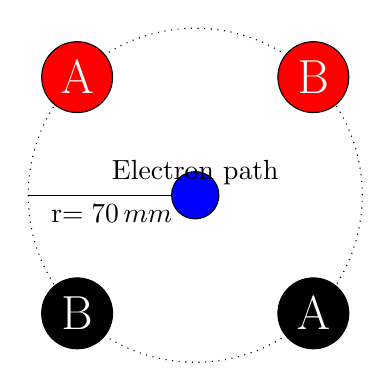
\begin{tikzpicture}
    \begin{scope}[scale=0.6]
        \draw[dotted] (0,0) circle (3.535);
        \draw (0,0) -- node[below] {r$=70\,\unit{mm}$} (-3.535, 0);

        \filldraw[fill=blue] (0,0) circle (0.5) node[above=0.3] {Electron path};

        \filldraw[fill=red] (2.5, 2.5) node[white] {\LARGE B} circle (0.75);
        \filldraw[fill=black] (-2.5, -2.5) node[white] {\LARGE B} circle (0.75);
        \filldraw[fill=red] (-2.5, 2.5) node[white] {\LARGE A} circle (0.75);
        \filldraw[fill=black] (2.5, -2.5) node[white] {\LARGE A} circle (0.75);
    \end{scope}
\end{tikzpicture}
\caption{Two pairs of current carrying wires (A and B) used to steer the electrons which are directed into the page. The current in the red wires is in the opposite direction to that in the black wires.}
\label{fig:mag_steering}
\end{figure}

Two pairs of steering coils, each with 25 turns, were constructed to implement this design. Each pair of wire bundles is connected to the other well away from the vacuum system to avoid disturbing the magnetic steering. The coils are mounted onto the vacuum system using plastic collars and the wires are confined in $20\,\unit{mm}$ electrical conduit.

In practise, typical currents to steer the electrons onto the detector are $1.76\,\unit{A}$ and $1.52\,\unit{A}$ for the two axes. These values are much higher than estimated but well within the capabilities of the device and its power supply.

\section{Optical Dipole Trap}

\subsection{Tapered Amplifier}
A \gls{ta} (see figure \ref{fig:tasetup}) serves as the light source for the \gls{odt}. It is constructed from an Eagleyard Photonics $780\,\unit{nm}$, $2\,\unit{Watt}$ semiconductor tapered amplifier (TA) \gls{ta} seeded by a homebuilt external cavity diode laser (ECDL). This method of seeding \glspl{ta} is known as a \gls{mopa} system\cite{wilson_narrow-linewidth_1998}. Due to a change in the mounting of the \gls{ta} chip it was necessary to redesign part of the group's \gls{mopa} hardware\cite{sheludko_shaped_2010}. A number of other changes to the original \gls{mopa} design were also made to allow greater flexibility during alignment. A new \gls{mopa} was constructed from the new and existing parts.

\begin{figure}[h]
\centering
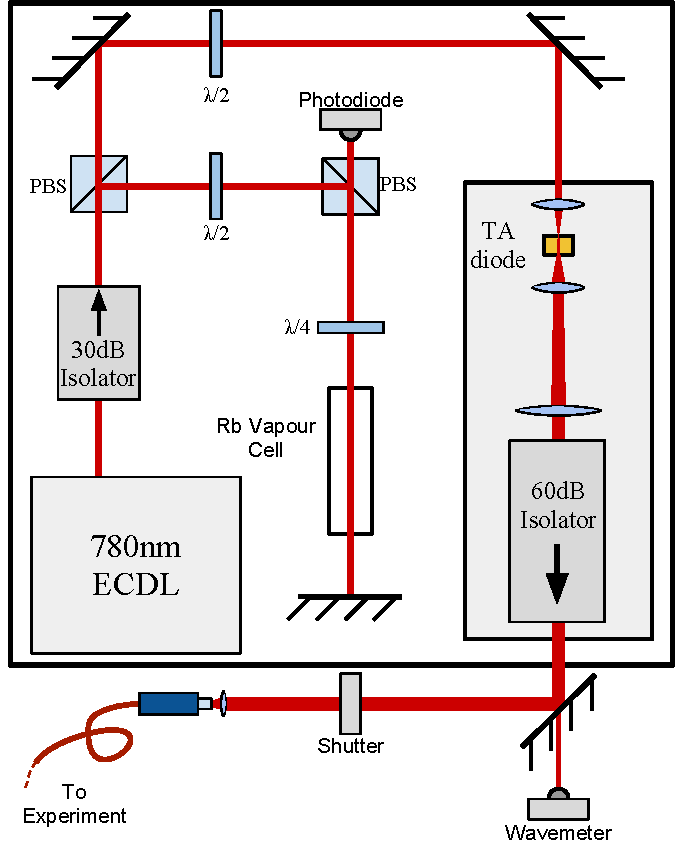
\includegraphics[width=0.5\textwidth]{figs/TAsetup.pdf}
\caption{The configuration of the light source for the ODT. The tapered amplifier (TA) is seeded by the external cavity diode laser (ECDL). A portion of the seed beam is directed into a saturated absorption setup. A tiny portion of the amplified beam transmits through the final mirror and is incident on the wavemeter. A computer controlled shutter is used to control the input to the fibre. The amplified beam has been coupled into a polarisation maintaining, single mode fibre.}
\label{fig:tasetup}
\end{figure}

The \gls{ecdl} provides approximately $25\,\unit{mW}$ of injection seed with a linewidth typically below $300\,\unit{kHz}$. The seed laser is focussed onto the input facet of the \gls{ta} with a high \gls{na} lens\footnote{Thorlabs C230TM-B f=$4.5\,\unit{mm}$ $0.55\,\unit{NA}$}. The beam from the output facet of the \gls{ta} is collimated with two lenses due to the high astigmatism in the output beam. The first lens is a high \gls{na} aspheric lens\footnote{Thorlabs C330TM-B f=$3.1\,\unit{mm}$ $0.68\,\unit{NA}$} and the second is a cylindrical lens\footnote{Unknown provenance f=$50\,\unit{mm}$} which counters the remaining horizontal divergence. The outgoing beam then passes through a double stage optical isolator which prevents optical feedback causing damage to the \gls{ta}. The maximum output power of the \gls{ta}, after the isolator, is $1.75\,\unit{W}$ when the \gls{ta} is run at a current of $4\,\unit{A}$.

A small portion of the seed beam is siphoned into a saturated absorption setup\cite{maguire_theoretical_2006, haroche_theory_1972, preston_doppler-free_1996} to allow locking of the seed beam to the resonances of rubidium. This is not particularly useful during normal operation since the laser must be detuned well beyond the resonances for use as an \gls{odt}, but locking to an atomic resonance is useful during the alignment process as discussed below.

The output beam is coupled into a polarisation maintaining, single-mode fibre with the output end located near the main experiment. The coupling efficiency at high power is approximately 40\%. Most of the power loss is due to the non-Gaussian profile of the \gls{ta} beam. While the significant power loss is detrimental to trap depth the major advantage of fibre coupling the beam is that the output beam is almost perfectly Gaussian in profile which is a necessity for \glspl{odt}.

A fraction of a percent of the light reflecting off the final mirror before the fibre mount transmits through the mirror. This light is incident on a wavemeter and is used to monitor the wavelength of the output beam as well as check that the light is of a single wavelength. Occasionally the seed laser will operate in two longitudinal modes simultaneously and the \gls{ta} amplifies both frequencies.

An old hard disc drive was used to create a shutter\cite{scholten_enhanced_2007}. The shutter has a response time lag of $6\,\unit{ms}$ which must be taken into account when scheduling the timing of the experiment.

The performance of the \gls{ta} is sensitive to temperature so it is maintained at a constant temperature with water cooling and a \gls{tec} controlled by a Thorlabs temperature controller\footnote{Thorlabs TED200 C}. The \gls{ecdl} is controlled and powered by a Moglabs Diode Laser Controller and the \gls{ta} is powered by a ThorLabs laser diode controller\footnote{Thorlabs LDC 240 C}.

\subsection{Optical Dipole Trap}

The output of the \gls{ta} fibre provides a Gaussian beam and the optics described in this section focus the beam in the region of the \gls{mot} atom cloud.

The output end of the \gls{ta} fibre is mounted in a cage to allow precise alignment of the focussing optics. Beam expansion and contraction lens pairs can be mounted into the cage and the final lens before the vacuum system or `objective' lens is also mounted here. While the potential for shrinking and expanding the beam incident on the objective lens is available it was not used in the final configuration.

There is a limited amount of optical access to the vacuum system and the \gls{odt} uses two almost orthogonal (each beam is approximately $35^{\circ}$ from vertical) beam paths the second of which is shared with the $480\,\unit{nm}$ ionisation laser. All the windows to the vacuum system are \gls{ar} coated for $780\,\unit{nm}$ light.

The distance from one window to the opposite is $412.3\,\unit{mm}$ and the \gls{mot} is situated halfway between them. One of the objective lenses\footnote{Thorlabs AC508-250-B-ML f=$250\,\unit{mm}$} has a focal length of $250\,\unit{mm}$ which gives sufficient space to allow for adjustments of the beam waists without touching the glass of the window. After the exit window of the first beam is another $250\,\unit{mm}$ lens to re-collimate the beam. This collimated beam is then propagated through free space to the second beam axis.

The second beam axis is shared with the blue, nanosecond-pulse ionisation laser. A long-pass dichroic mirror\footnote{Thorlabs DMLP567L} is used to combine the two beam paths. The focussing optics for the ionisation and the \gls{odt} are located before the dichroic. The objective lens for the second beam of the \gls{odt} is a $300\,\unit{mm}$ lens\footnote{Thorlabs AC508-300-B-ML f=$300\,\unit{mm}$} due to the extra distance imposed by the dichroic.

As mentioned in \ref{odt_polarisation} the polarisation of the second beam must be orthogonal to that of the first to avoid standing waves and this is achieved with a half-waveplate as indicated in figure \ref{fig:dipole_rig}.

After the second trapping beam has left the vacuum system it is incident on a power meter. The power meter operates with a reflective attenuator and the reflected beam is incident on a photodiode that is used for timing measurements. The final reflection off the photodiode is safely disposed of with a beam stop.

\begin{figure}[h]
\centering
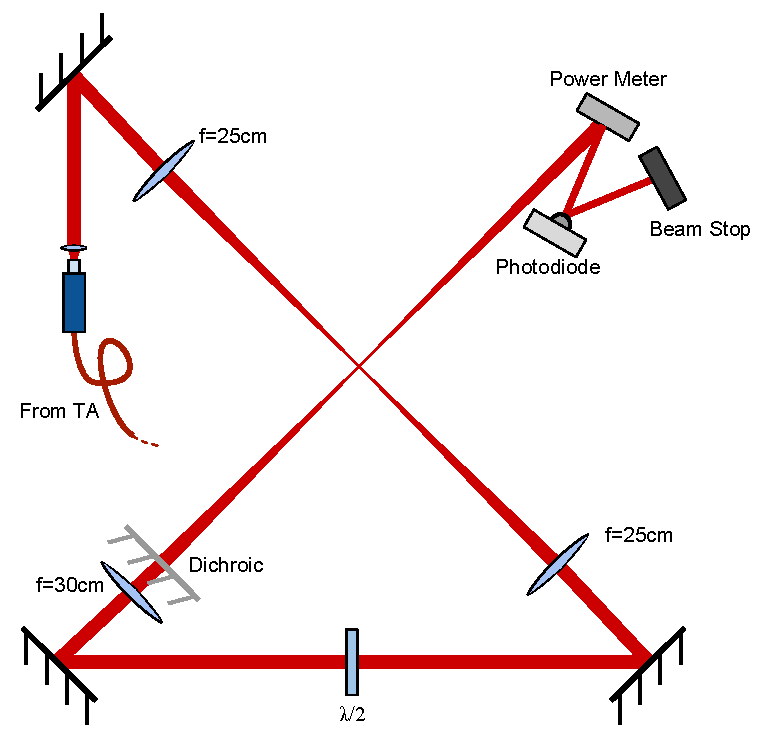
\includegraphics[width=0.4\textwidth]{figs/DipoleTrapRig.pdf}
\caption{The ODT beam path originates with the output of the TA fibre. The beam is then focussed by an objective lens and passed through the vacuum system with the beam waist at the MOT. As the beam leaves the vacuum system it is re-collimated and recycled for the second beam of the ODT. The polarisation is rotated with a half-waveplate and the beam is again focussed at the MOT. The beam also passes through a dichroic mirror so that the optical access can be shared with the blue ionisation beam. A power meter and photodiode located at the end of the beam path allow for diagnostics and the beam is terminated with a beam stop.}
\label{fig:dipole_rig}
\end{figure}

\subsubsection{Alignment}

The alignment of the crossed \gls{odt} is done by first tuning the seed \gls{ecdl} close to resonance such that when the laser is scanning the saturated absorption signal is visible on the oscilloscope. With small detuning the scattering rate becomes very large and portions of the \gls{mot} are visibly affected by the \gls{odt} beams when viewed by the \gls{ccd} cameras that monitor fluorescence. An example of this is shown in figure \ref{fig:mot_slice}. The level of effect the \gls{odt} beams have on the trapped atoms can be varied by altering their power and detuning. By altering the alignment of the the two \gls{odt} beams while observing the effects on the \gls{mot} the beam can be overlapped in the region of the \gls{mot}.

\begin{figure}[H]
\centering
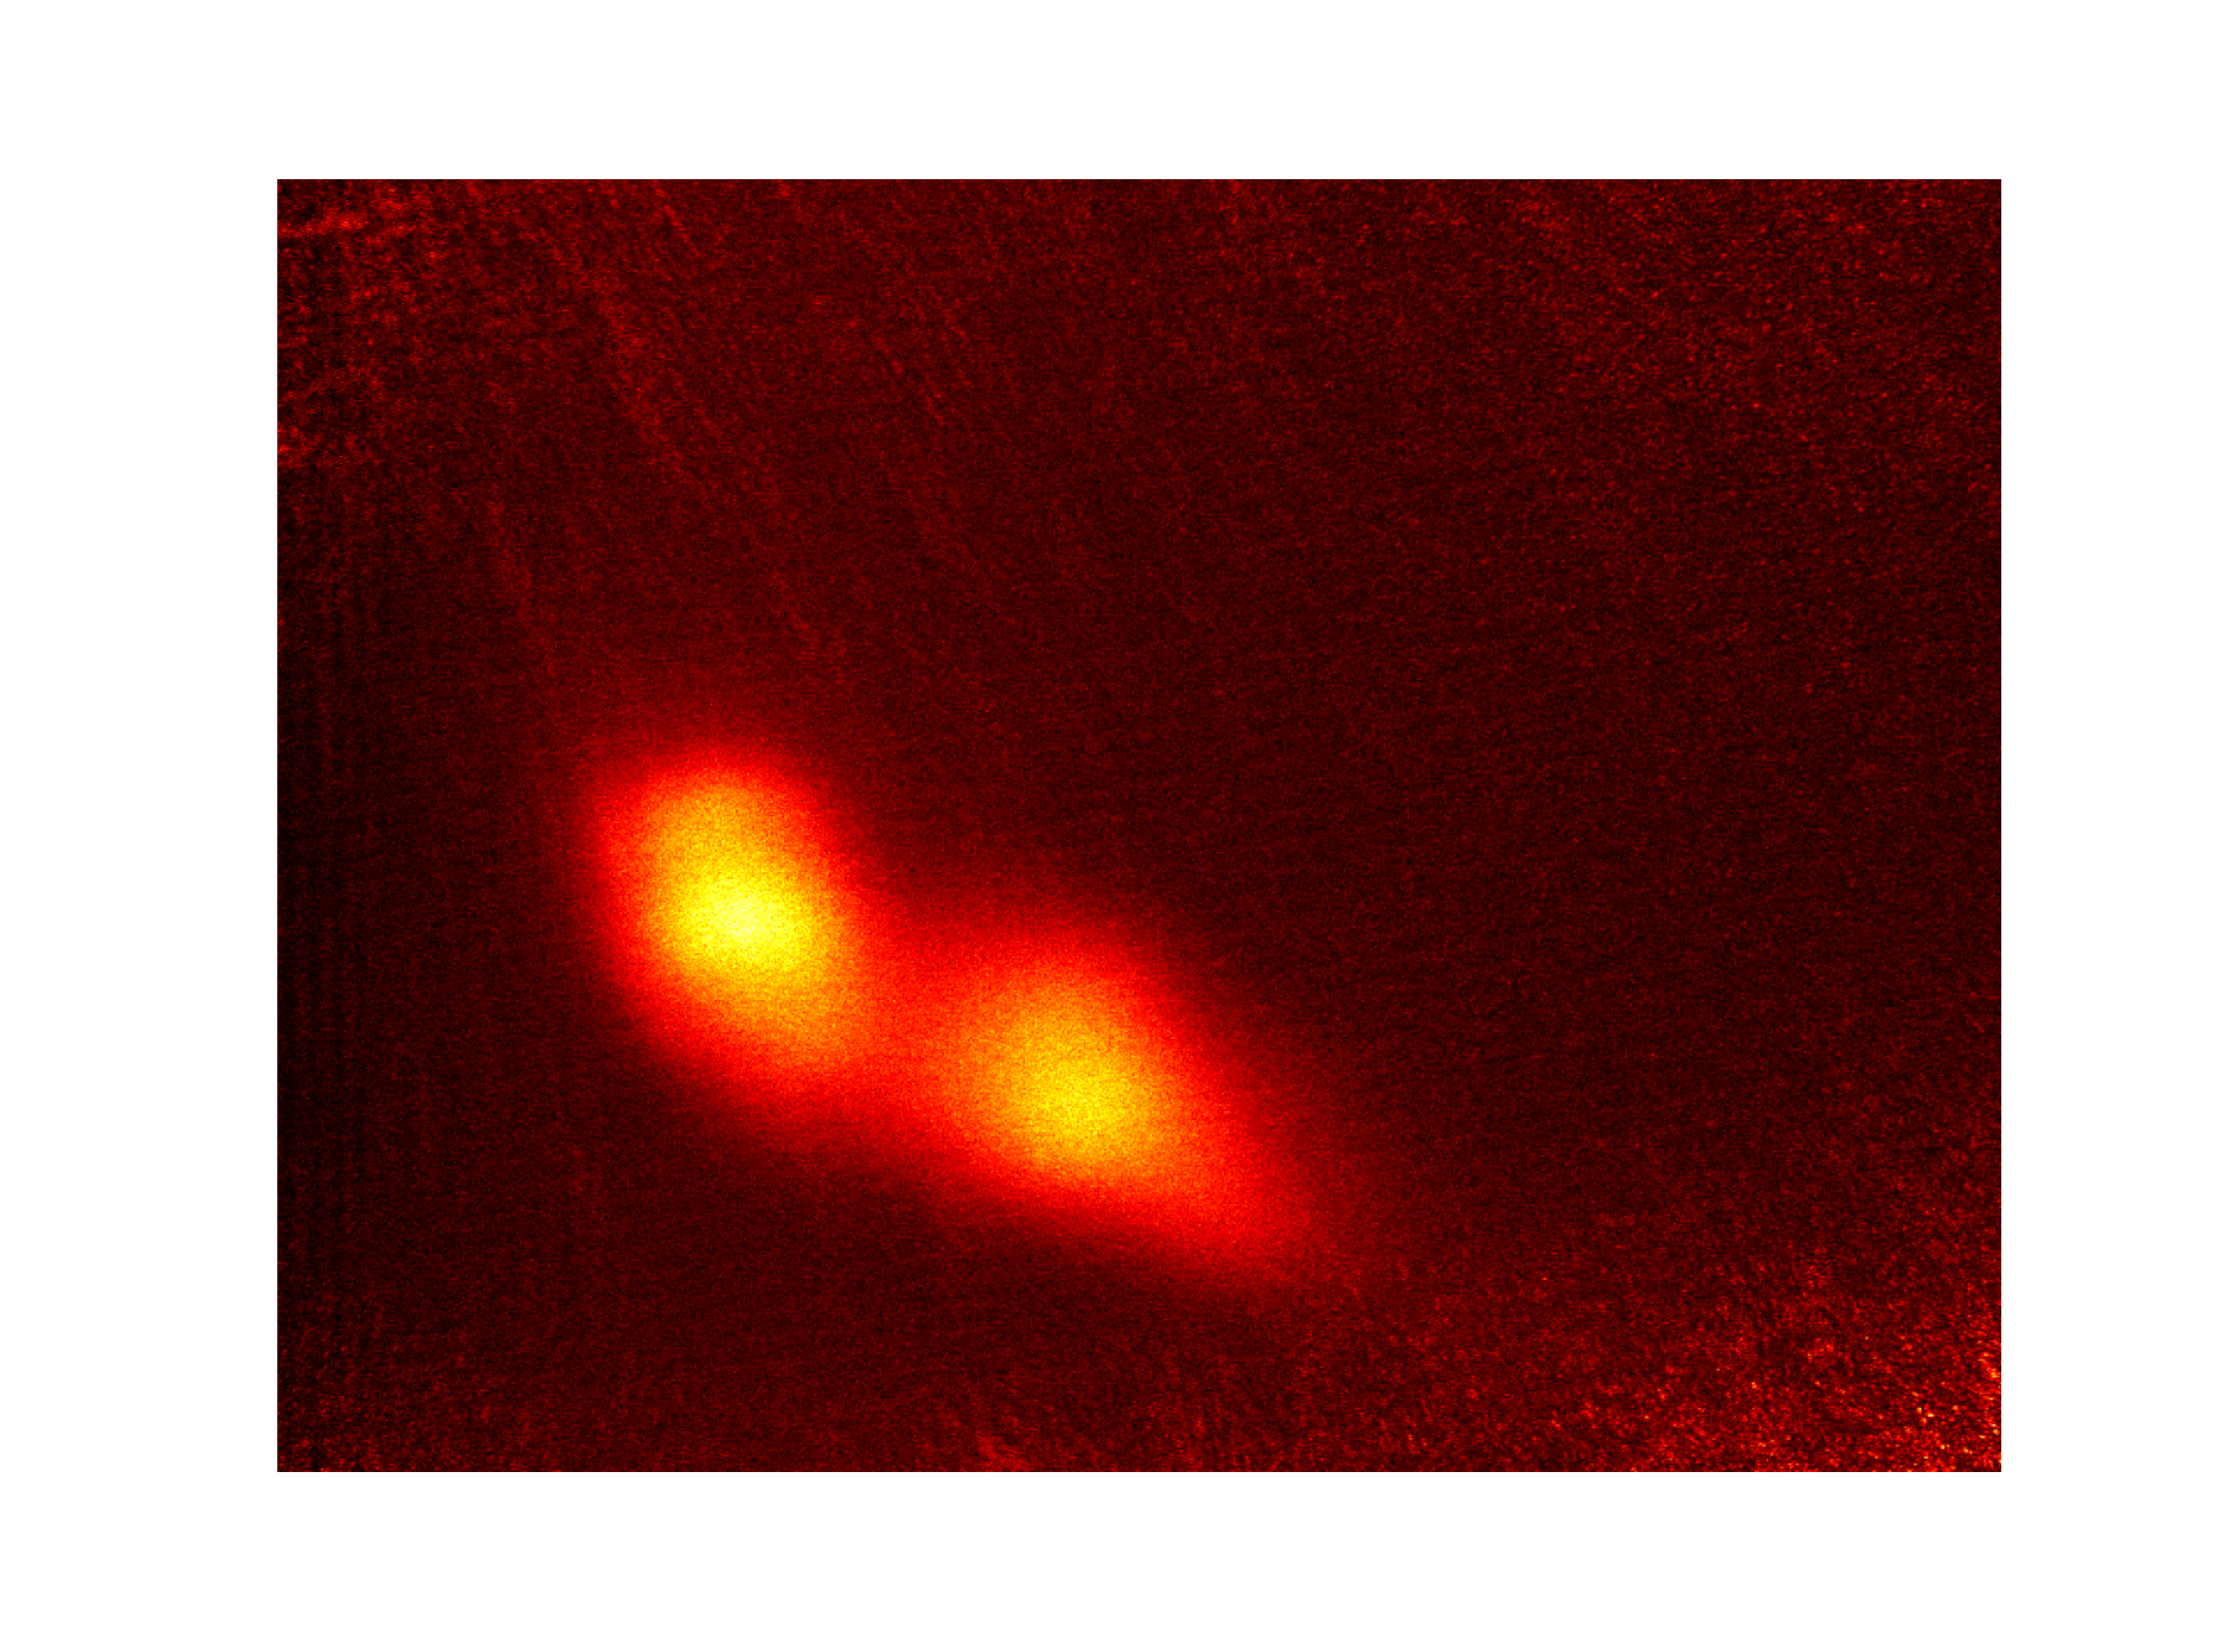
\includegraphics[width=0.3\textwidth]{figs/mot_slice.pdf}
\caption{The first beam of the ODT dividing the MOT atom cloud into two halves.}
\label{fig:mot_slice}
\end{figure}

\section{Absorption Imaging}

In order to detect trapping within the \gls{odt} it is necessary to have a way of imaging it. Fluorescence imaging is not sufficient due to the fact that the detuned beams of the \gls{odt} do not induce visible amounts of fluorescence. Absorption imaging was implemented to image the atoms in the \gls{odt}.

The light source for imaging is shared with the continuous excitation beam and is an \gls{ecdl} frequency stabilised with saturated absorption and controlled by a Mogbox\footnote{Moglabs DLC-202}. The power available for imaging can vary from a few microWatts to $2.5\,\unit{mW}$ depending on the position of the half wave plate located before the \gls{pbs} that splits the beam between the imaging and excitation beam lines. The imaging beam is then coupled into a fibre and brought over to the main experiment.

The imaging beam shares optical access with the vertical \gls{mot} beam. By putting the imaging beam slightly off axis compared to the \gls{mot} beam it is possible to insert and extract the beam without impact on the trapping beam.

A camera lens\footnote{Nikon AF Micro-Nikkor $200\,\unit{mm}$} is used to focus the beam onto a \gls{ccd} camera\footnote{Allied Vision Technologies Stingray F-080B}. The effective size of a camera pixel was calibrated by imaging a ruler at the same distance from the camera as the \gls{mot}. In this imaging beamline the effective pixel size was calculated to be $12.8\pm0.4\times12.8\pm0.4\,\unit{\mu m^2}$.

\begin{figure}[h]
\centering
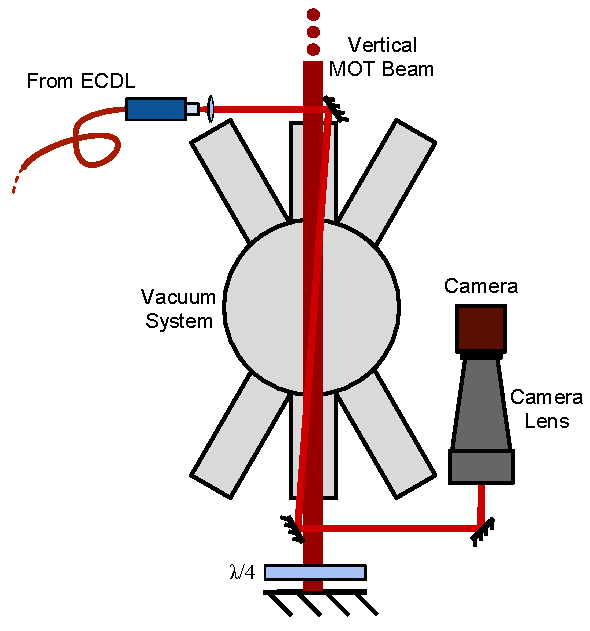
\includegraphics[width=0.5\textwidth]{figs/ImagingRig.pdf}
\caption{The imaging beam's optical access is shared with the vertical MOT beam. The beam is collimated from a fibre and is slightly off axis from the MOT beam. It is recorded by a Stingray CCD camera after being focussed by a Nikon camera lens.}
\label{fig:imaging_rig}
\end{figure}

The axis of the imaging beam is not ideal. The imaging beam axis would be orthogonal to both of the trapping beams to allow for clear images of both beams. Having the imaging axis orthogonal to gravity would also allow the observation of atom clouds falling. Unfortunately it is not currently feasible to put the imaging beam on the horizontal axis, due to the scarcity of optical access on that axis and the crowded nature inside the vacuum system. As the results in chapter 4 show it is still possible to differentiate between the two beams due to the off-axis alignment of the imaging beam.

For standard absorption images, an image with no atoms present is used as $I_0$ and an image with atoms creating a shadow is used as $I$ in equation \ref{eq:transmission_function_1}. For images of the \gls{odt} however the thermally expanding \gls{mot} is still visible so an image of the \gls{mot} is used as a background such that the \gls{odt} to be the only feature in the resulting absorption image.

\section{Software}

To perform absorption imaging new software was required to communicate with the AVT camera and to do the image analysis. This new software was created in Labview and Python.

The software for image acquisition, integration and absorption imaging was created in Labview and is able to acquire images from the camera in real time and apply the theory described in section \ref{sec:absorption_imaging} in order to immediately present the user with the absorption images (such as the one in figure \ref{fig:absorption_example}). The Labview software is also able to present the atom count for a given absorption image. More in-depth analysis, such as temperature measurements, is performed using Python programs described in more detail in chapter 4.

\section{Experimental Procedure}

During standard operation the \gls{caes} operates at a frequency of $10\,\unit{Hz}$. This cycle consists of:
\begin{enumerate}
\item Loading  the \gls{mot} for approximately $93\,\unit{ms}$.
\item Turning off the magnetic and optical trapping.
\item Turning on the excitation laser (\gls{cw}).
\item $5\,\unit{ns}$ ionisation pulse.
\item Turning on the accelerating electric field for $60\,\unit{\mu s}$.
\item Turning off the excitation laser and turning the magnetic and optical trapping back on.
\end{enumerate}

When aligning, imaging and configuring the \gls{odt} the process changes. The sequence now operates at approximately $2\,\unit{Hz}$ so that the absorption imaging software does not lag. The ionisation and acceleration steps are not necessary and more steps are required for imaging. The state of each of the lasers and coils during this process is shown in figure \ref{fig:sequence}.

The longest step is the loading of the \gls{mot} which requires both the Zeeman and \gls{mot} cooling. The \gls{odt} beam is also on during this stage so that the \gls{odt} can load. This step lasts for approximately $300\,\unit{ms}$ so that the \gls{mot} has plenty of time to load. 

In the next step atoms are held solely by the \gls{odt}. This length of this step varies depending on what is being examined. By imaging after a certain delay snapshots of the \gls{odt}'s evolution can be made.

In the imaging step the imaging laser is turned on and camera is triggered. It is important to turn the \gls{mot} repump laser on so that atoms do not fall into the dark state. With high intensity and small detuning, the \gls{odt} laser acts as a repump and excitation laser itself. The \gls{odt} is turned off during imaging.

\begin{figure}[H]
\centering
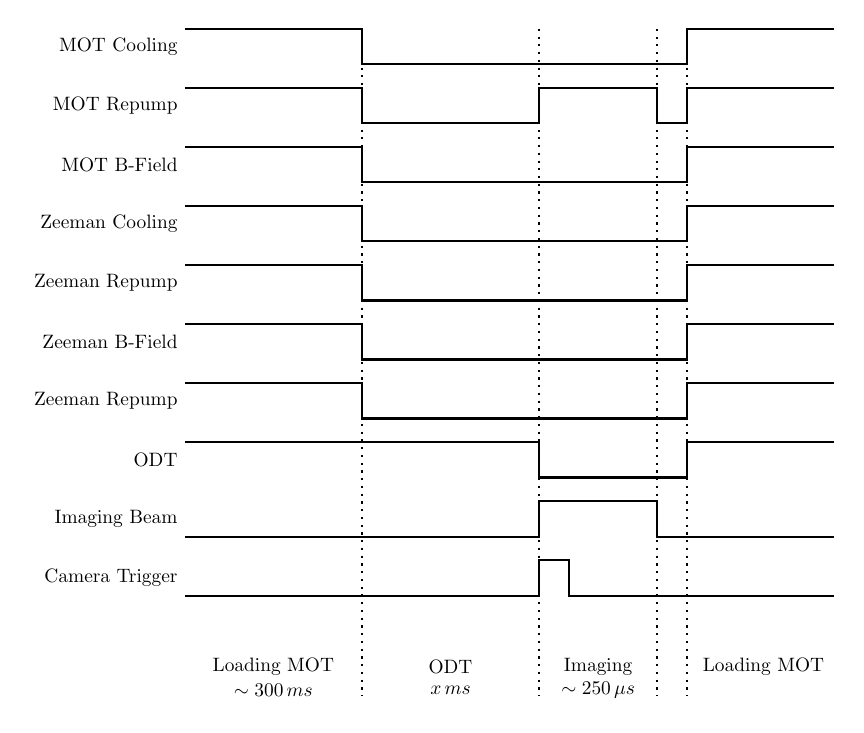
\begin{tikzpicture}[scale=0.75, every node/.style={scale=0.7}]
    \begin{scope}[thick, decoration={snake,amplitude=.4mm,
        segment length=2mm,post length=1mm}]
      \draw (0,10) node[left] {MOT Cooling};
        \draw (0,10.3)  -- (3, 10.3) -- (3, 9.7) -- (8.5, 9.7) -- (8.5, 10.3) -- (11, 10.3);

      \draw (0, 9) node[left] {MOT Repump};
        \draw (0, 9.3) -- (3, 9.3) -- (3, 8.7) -- (6, 8.7) -- (6, 9.3) -- (8, 9.3) -- (8, 8.7) -- (8.5, 8.7) -- (8.5, 9.3) -- (11, 9.3);

      \draw (0, 8) node[left] {MOT B-Field};
        \draw (0, 8.3) -- (3, 8.3) -- (3, 7.7)-- (8.5, 7.7) -- (8.5, 8.3) -- (11, 8.3);

      \draw (0, 7) node[left] {Zeeman Cooling};
        \draw (0, 7.3) -- (3, 7.3) -- (3, 6.7) -- (8.5, 6.7) -- (8.5, 7.3) -- (11, 7.3);

      \draw (0, 6) node[left] {Zeeman Repump};
        \draw (0, 6.3) -- (3, 6.3) -- (3, 5.7) -- (8.5, 5.7) -- (8.5, 6.3) -- (11, 6.3);

      \draw (0, 5) node[left] {Zeeman B-Field};
        \draw (0, 5.3) -- (3, 5.3) -- (3, 4.7) -- (8.5, 4.7) -- (8.5, 5.3) -- (11, 5.3);

      \draw (0, 4) node[left] {Zeeman Repump};
        \draw (0, 4.3) -- (3, 4.3) -- (3, 3.7) -- (8.5, 3.7) -- (8.5, 4.3) -- (11, 4.3);

      \draw (0, 3) node[left] {ODT};
        \draw (0, 3.3) -- (6, 3.3) -- (6, 2.7) -- (8.5, 2.7) -- (8.5, 3.3) -- (11, 3.3);

      \draw (0, 2) node[left] {Imaging Beam};
        \draw (0, 1.7) -- (6, 1.7) -- (6, 2.3) -- (8, 2.3) -- (8, 1.7) -- (11, 1.7);

      \draw (0, 1) node[left] {Camera Trigger};
        \draw (0, 0.7) -- (6, 0.7) -- (6, 1.3) -- (6.5, 1.3) -- (6.5, 0.7) -- (11, 0.7);

    \draw[dotted] (3, 10.3) -- (3, -1);
    \draw (1.5, -0.5) node {Loading MOT};
    \draw (1.5, -0.9) node {$\sim300\,\unit{ms}$};

    \draw[dotted] (6, 10.3) -- (6, -1);
    \draw (4.5, -0.5) node {ODT};
    \draw (4.5, -0.9) node {$x\,\unit{ms}$};

    \draw[dotted] (8, 10.3) -- (8, -1);
    \draw (7, -0.5) node {Imaging};
    \draw (7, -0.9) node {$\sim250\,\unit{\mu s}$};


    \draw[dotted] (8.5, 10.3) -- (8.5, -1);
    \draw (9.8, -0.5) node {Loading MOT};
    \end{scope}
\end{tikzpicture}
\caption{The experimental sequence used to examine the ODT.}
\label{fig:sequence}
\end{figure}

Another important consideration is the delay between a change in a control signal and response from a device (such as a laser, magnetic coil or camera). Lasers that are controlled with \glspl{aom} have a very fast response time of order microseconds. The response time of the AVT camera has not been measured however it is significantly less than the usual $30-100\,\unit{\mu s}$ exposure time of the camera. The response times of the mechanical shutters used on the Zeeman slower and \gls{odt} however are significant.

The response times of the shutters can easily be measured by using a photodiode to compare the amount of light transmitting through the shutters with the signal controlling the shutter. This method has shown that the response time of the Zeeman slower shutter is $4.6\,\unit{ms}$ and the \gls{odt} shutter is $6.2\,\unit{ms}$. These values were used when scheduling the timing of the experiment.

\chapter{Results}

If I ever get any results go in here.

\section{absorption images of the mot}

    \subsection{Temperature}

    \subsection{Atom Count}

\section{absorption images of ODT}

    \subsection{Atom Count}

    \subsubsection{Lifetime}


\printglossaries
\newpage

\bibliography{bib}{}
\bibliographystyle{unsrt}


\end{document}
